%
% exemplo genérico de uso da classe iiufrgs.cls
% $Id: iiufrgs.tex,v 1.1.1.1 2005/01/18 23:54:42 avila Exp $
%
% This is an example file and is hereby explicitly put in the
% public domain.
%
\documentclass[cic,resumo-unibral]{iiufrgs}
% Para usar o modelo, deve-se informar o programa e o tipo de documento.
% Programas :
% * cic       -- Graduação em Ciência da Computação
% * ecp       -- Graduação em Ciência da Computação
% * ppgc      -- Programa de Pós Graduação em Computação
% * pgmigro   -- Programa de Pós Graduação em Microeletrônica
%
% Tipos de Documento:
% * tc                -- Trabalhos de Conclusão (apenas cic e ecp)
% * diss ou mestrado  -- Dissertações de Mestrado (ppgc e pgmicro)
% * tese ou doutorado -- Teses de Doutorado (ppgc e pgmicro)
% * ti                -- Trabalho Individual (ppgc e pgmicro)
% * resumo-unibral    -- Resumo estendido anexado a TC realizado na TU Berlin
%
% Outras Opções:
% * english    -- para textos em inglês
% * openright  -- Força início de capítulos em páginas ímpares (padrão da
% biblioteca)
% * oneside    -- Desliga frente-e-verso
% * nominatalocal -- Lê os dados da nominata do arquivo nominatalocal.def


% Use unicode
\usepackage[utf8]{inputenc}   % pacote para acentuação

% Necessário para incluir figuras
\usepackage{graphicx}         % pacote para importar figuras
\graphicspath{ {img/} }

\usepackage{times}            % pacote para usar fonte Adobe Times
% \usepackage{palatino}
% \usepackage{mathptmx}       % p/ usar fonte Adobe Times nas fórmulas

\usepackage{float}
\setlength{\intextsep}{1\baselineskip} % evita espaços antes e depois de floats
\setlength{\belowcaptionskip}{10pt plus 3pt minus 2pt} % espaço depois de caption
\usepackage{amssymb}

% Para algoritmos
\usepackage{amsfonts}
\usepackage{algpseudocode}
\usepackage{algorithm}
\usepackage{algorithmicx}

\usepackage[alf,abnt-emphasize=bf]{abntex2cite}	% pacote para usar citações abnt

%
% Informações gerais
%
\title{Towards Synchronizing Relations Between Artifacts in the Java Technological Space}

\author{Bombardelli da Silva}{William}
% alguns documentos podem ter varios autores:
% \author{Flaumann}{Frida Gutenberg}
% \author{Flaumann}{Klaus Gutenberg}

% orientador e co-orientador são opcionais (não diga isso pra eles :))
\advisor[Prof.ª Dra.]{Ribeiro}{Leila}
\def\advisornameBR{Orientadora brasileira}
\advisorDE[Dr.-Ing.]{Trollmann}{Frank}

% a data deve ser a da defesa; se nao especificada, são gerados
% mes e ano correntes
% \date{maio}{2001}

% o local de realização do trabalho pode ser especificado (ex. para TCs)
% com o comando \location:
% \location{Itaquaquecetuba}{SP}

% itens individuais da nominata podem ser redefinidos com os comandos
% abaixo:
% \renewcommand{\nominataReit}{Prof\textsuperscript{a}.~Wrana Maria Panizzi}
% \renewcommand{\nominataReitname}{Reitora}
% \renewcommand{\nominataPRE}{Prof.~Jos{\'e} Carlos Ferraz Hennemann}
% \renewcommand{\nominataPREname}{Pr{\'o}-Reitor de Ensino}
% \renewcommand{\nominataPRAPG}{Prof\textsuperscript{a}.~Joc{\'e}lia Grazia}
% \renewcommand{\nominataPRAPGname}{Pr{\'o}-Reitora Adjunta de P{\'o}s-Gradua{\c{c}}{\~a}o}
% \renewcommand{\nominataDir}{Prof.~Philippe Olivier Alexandre Navaux}
% \renewcommand{\nominataDirname}{Diretor do Instituto de Inform{\'a}tica}
% \renewcommand{\nominataCoord}{Prof.~Carlos Alberto Heuser}
% \renewcommand{\nominataCoordname}{Coordenador do PPGC}
% \renewcommand{\nominataBibchefe}{Beatriz Regina Bastos Haro}
% \renewcommand{\nominataBibchefename}{Bibliotec{\'a}ria-chefe do Instituto de Inform{\'a}tica}
% \renewcommand{\nominataChefeINA}{Prof.~Jos{\'e} Valdeni de Lima}
% \renewcommand{\nominataChefeINAname}{Chefe do \deptINA}
% \renewcommand{\nominataChefeINT}{Prof.~Leila Ribeiro}
% \renewcommand{\nominataChefeINTname}{Chefe do \deptINT}

% A seguir são apresentados comandos específicos para alguns
% tipos de documentos.

% Relatório de Pesquisa [rp]:
% \rp{123}             % numero do rp
% \financ{CNPq, CAPES} % orgaos financiadores

% Trabalho Individual [ti]:
% \ti{123}     % numero do TI
% \ti[II]{456} % no caso de ser o segundo TI

% Monografias de Especialização [espec]:
% \espec{Redes e Sistemas Distribuídos}      % nome do curso
% \coord[Profa.~Dra.]{Weber}{Taisy da Silva} % coordenador do curso
% \dept{INA}                                 % departamento relacionado

%
% palavras-chave
% iniciar todas com letras minúsculas, exceto no caso de abreviaturas
%
\keyword{Sincronização de Modelos}
\keyword{Metamodelos Java}
\keyword{Rede de Modelos}
\keyword{Transformação de Modelos}
\keyword{Desenvolvimento Orientado a Modelos}
\keyword{Engenharia de Software}

%\settowidth{\seclen}{1.10~}

%
% inicio do documento
%
\begin{document}

% folha de rosto
% às vezes é necessário redefinir algum comando logo antes de produzir
% a folha de rosto:
% \renewcommand{\coordname}{Coordenadora do Curso}
\maketitle

% dedicatoria
% \clearpage
% \begin{flushright}
%     \mbox{}\vfill
%     {\sffamily\itshape
%       ``If I have seen farther than others,\\
%       it is because I stood on the shoulders of giants.''\\}
%     --- \textsc{Sir~Isaac Newton}
% \end{flushright}

% agradecimentos
%\chapter*{Agradecimentos}
%Agradeço ao \LaTeX\ por não ter vírus de macro\ldots


\begin{abstract}
O uso de modelos em processos de engenharia de software tem crescido nos últimos anos. Ao passo que o uso cresce, cresce também a relevância de alguns problemas relacionados à área. Um deles é o problema de sincronização de modelos, que consiste basicamente em manter todos os modelos de uma aplicação de software consistentes entre si. Em outras palavras, os modelos de um software tendem a ser mudados ao longo do seu tempo de vida, e quando isto acontece, estas mudanças têm que ser devidamente despachadas a todos os modelos. Para aplicações de software de grande porte é inviável realizar tal procedimento de sincronização manualmente, portanto, é desejado a criação de métodos automáticos capazes de sincronizar os modelos do software.

Não exploramos este problema para qualquer tipo de software, ao invés disso limitamos nosso domínio ao espaço tecnológico Java, de maneira que o escopo deste trabalho permaneça factível. Esta tese procede portanto (1) identificando e definindo formalmente alguns modelos do espaço tecnológico Java, (2) identificando e formalizando algumas relações entre eles, criando uma rede de metamodelos a ser mantida sincronizada, e mostrando como estas relações trabalham através de um caso representativo, e finalmente (3) discutindo a sincronização desta rede de metamodelos. Os resultados incluem a implementação destas relações mais o relatório sobre a experiência de desenvolver isso neste trabalho de conclusão de curso.
\end{abstract}


\begin{extendedsummary}

\section{Introdução}
Os últimos avanços relacionados a técnicas de engenharia de software incluem a chamada \textbf{engenharia orientada a modelos} (inglês: Model-driven Engineering ou MDE), sinônimo para \textbf{desenvolvimento orientado a modelos} (inglês: Model-driven Development ou MDD), onde modelos de software são os artefatos primários do desenvolvimento do software. Em MDE, um sistema de software tem possivelmente diversos modelos abstraindo-o, cada um representando certos aspectos de todo o sistema. Esses modelos têm relações entre si, no sentido de que devem descrever o sistema consistentemente, não apresentando contradições lógicas. Exemplos de modelos de software são \emph{diagramas de classes UML}, \emph{diagramas de casos de uso} ou até mesmo código-fonte. Muito embora o uso de modelos pode contribuir positivamente para o desenvolvimento de aplicações de software, ele também introduz alguns problemas, entre eles está o \textbf{problema de sincronização de modelos}, que consiste basicamente em manter todos os modelos de um software consistentes entre eles mesmos. Em outras palavras, ao passo que uma aplicação de software evolui, seus modelos sofrem alterações que devem ser encaminhadas corretamente a todos os outros modelos relacionados a esta aplicação \cite{diskin2011model}.

Propõe-se então neste trabalho uma abordagem ao problema baseada na criação de uma \textbf{rede de modelos interconectados}, que deve ser mantida consistente, i.e. todos os modelos devem estar sincronizados. Para exemplificar, suponha um \emph{diagrama de classes UML}, uma séria de \emph{diagramas de sequência UML} e um código-fonte. Se um método tem seu nome alterado no diagrama de classes, todas as ocorrências deste método devem ter seus nomes atualizados nos diagramas de sequência e no código-fonte. Acontece, porém, que uma ferramenta de sincronização de modelo automática e genérica capaz de ser aplicada na prática não é conhecida por nós, apesar de que um esforço expressivo tem sido feito pela comunidade acadêmica para criar solução para este problema.

O objetivo amplo deste trabalho é explorar o problema de sincronização de modelos, analisando modelos e suas relações com outros modelos e estabelecendo técnicas de sincronização. Todavia, para manter o escopo factível, restringimos o domínio ao \textbf{espaço tecnológico Java} e fixamos as seguintes metas: (1) apresentar e definir formalmente alguns \textbf{modelos} do espaço tecnológico Java; (2) formalizar e explicar algumas \textbf{relações} entre esses modelos, criando uma rede de metamodelos. e (3) discutir como \textbf{sincronização} pode ser alcançada nessa rede. Está fora, portanto, do escopo deste trabalho a criação de definições completas de metamodelos ou a implementação de um algoritmo totalmente funcional de sincronização, assim como uma análise teórica profunda do problema ou da performance das relações desenvolvidas. Contudo, os resultados deste trabalho contribuem para um melhor intendimento do problema de sincronização de modelos de espaços tecnológicos complexos.

\section{Fundamentação}
Abaixo está o resumo de algumas definições importantes para o restante do texto.

\subsection{Modelos}
De acordo com \citet{favre2004foundations}, um sistema é o elemento de discurso principal ao falar de MDE. Um modelo é um sistema que representa um outro sistema. Um modelo é expresso usando uma linguagem de modelagem, que por sua vez nada mais é que um conjunto de todos os modelos expressados naquela linguagem. Por final, um metamodelo é então um modelo de uma linguagem de modelos, isto é ele especifica o que pode ser escrito usando uma certa linguagem. Um modelo $M$ está em conformidade com um metamodelo $MM$, se e somente se, $M$ pertence à linguagem especificada po $MM$ \cite{favre2004foundations2}.

\subsection{Sincronização de Modelos}
Uma relação de modelos é definida aqui abstratamente como qualquer relacionamento ou restrição possível de acontecer entre um modelo fonte e um modelo alvo. Sincronização de modelos pode ser vista como uma função $s : M \times M \times \Delta_M \times N \times N \times \Delta_N \rightarrow M \times N $, onde $s(m_0,m_1,\delta_m,n_0,n_1,\delta_n) = (m_2,n_2)$ significa que os modelos sincronizados $m_2$ e $n_2$ são criados a partir dos modelos inicialmente sincronizados $m_0$ e $n_o$ e os modelos modificados não sincronizados $m_1$ e $n_1$, considerando as modificações (respectivamente $\delta_m$ e $\delta_n$) executadas sobre ambos \cite{diskin2011model}. Uma rede de modelos de um sistema $S$ é um grafo não-direcionado $G = (V,E)$, onde cada vértice $v_i \in V$ representa um modelo único $i$ abstraindo $S$, e uma aresta $\{v_i, v_j\}$ existe se, e somente se, há uma relação entre ambos os modelos $i$ e $j$.

\subsection{Gramática de Grafos Triplos}
Com o uso de um grafo triplo, uma relação entre um modelo fonte $S$ e um modelo alvo $T$ é abstraída em uma tripla $(G^S,G^C,G^T)$ – onde $G^S$ é a representação em grafo dos elementos do modelo fonte, $G^T$ é a representação dos elementos do modelo alvo, e $G^C$ representa a correspondência entre os dois conjuntos de elementos – juntamente com dois mapeamentos $s_G: G^C \rightarrow G^S$ e $t_G: G^C \rightarrow G^T$, que conectam os três grafos \citep{hermann2011correctness}. Neste caso, uma adição no grafo triplo $G = (G^S,G^C,G^T)$, que leva a um novo grafo triplo $H = (H^S,H^C,H^T)$, consiste em um morfismo de grafo triplo $m: G \rightarrow H$, com $m = (m^S,m^C,m^T)$, de acordo com a Figura \ref{fig:tg_morphism}.
\begin{figure}[h]
	\centering
	\caption{O morfismo $m: G \rightarrow H$ é um grafo triplo $m =  (m^S,m^C,m^T)$.}
	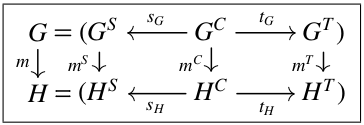
\includegraphics[width=15em]{tg_morphism}\\
	Fonte: \citep{hermann2011correctness}
	\label{fig:tg_morphism}
\end{figure}

Uma regra tripla é um morfismo de grafo triplo $t = (t^S,t^C,t^T) : L \rightarrow R$. Um axioma triplo é uma regra tripla $t_a = (t^S,t^C,t^T) : \varnothing \rightarrow R$ \cite{ehrig2007information}. Uma gramática de grafo triplo(inglês: Triple Graph Grammar ou TGG) $TGG = (t_a, T_{rules})$ consiste de um axioma triplo $t_a$ e um conjunto de regras triplas $T_{rules}$ \cite[p. 4]{giese2010toward}. Grafos triplos são utilizados neste trabalho como descrição de uma relação entre dois metamodelos, enquanto que TGGs descrevem uma espécie de linguagem da relação consistente entre estes dois metamodelos. Entretanto, regras extras podem ser derivadas de uma TGG para criar a semântica operacional do procedimento de sincronização da relação \cite{giese2010toward}.

\section{Relações de Metamodelos no Espaço Tecnológico Java}

Foi selecionado neste trabalho um conjunto de metamodelos típicos do espaço tecnológico Java e foram identificadas relações entre eles, criando-se assim uma \textbf{rede de metamodelos}. Dessa rede, quatro metamodelos e suas relações são trabalhadas mais profundamente, a saber \textit{Java}, \textit{UMLClassDiagram}, \textit{UMLSequenceDiagram} e \textit{UMLContract}.

Um modelo \textbf{\textit{Java}} (i.e. o código-fonte) contem informações tanto estruturais quanto comportamentais, e por isso se relaciona com os outros três metamodelos analisados. O metamodelo \textit{Java} criado não é completo, pois não modela toda a gramática da linguagem Java, entretanto aspectos arquiteturais de um programa orientado a objetos (e.g. classes, interfaces, métodos, atributos, etc.) são representados. O metamodelo \textbf{\textit{UMLClassDiagram}} é construído a partir dos conceitos de classe, propriedade, operação, interface e pacote. Ele é usado para descrever a estrutura de um programa orientado a objetos e sua relação com o metamodelo \textit{Java} é dado por uma tradução quase direta entre seus elementos.

Para representar alguns aspectos comportamentais,\textbf{ \textit{UMLSequenceDiagram}} é usado, dado que um diagrama de sequência representa tempos-de-vida de objetos e mensagens trocadas entre eles. No modelo \textit{Java} isto pode ser representado por chamadas de métodos entre classes ou por anotações sobre métodos, representando a ordem em que as trocas de mensagens ocorrem. Portanto, na nossa abordagem, cada \textit{linha-de-vida} (\textit{lifeline}) representa o comportamento de um método Java e cada mensagem enviada a partir desta \textit{linha-de-vida} é modelada em uma anotação (\textit{Java annotation}) sobre o respectivo método, que codifica a metainformação da ordem de chamadas a outros métodos.

O metamodelo \textbf{\textit{UMLContract}} é baseado nas ideias de programação por contrato, onde operações têm restrições (\textit{constraints}) de pré e pós-condição assim como de invariante. Sua relação com \textit{Java} é que cada restrição dos contratos pode ser (1) testada através de asserções (\textit{assertions}) e (2) expressa em termos de anotações no modelo \textit{Java}. Além disso, pode-se ter métodos de checagem de consistência interna de classe que verificam as restrições da classe e, portanto, devem ser mantidas sincronizadas com os modelos de \textit{UMLContract} (i.e. os contratos). Desta maneira, as relações desenvolvidas neste trabalho estabelecem que cada restrição de \textit{UMLContract} corresponde a uma anotação (sobre um método ou atributo) de \textit{Java}, assim como uma asserção pertencente a um método de checagem da classe.

As três relações comentadas acima (\textit{UMLClassDiagram2Java}, \textit{UMLSequenceDiagram2Java} e \textit{UMLContract2Java}) foram desenvolvidas usando TGGs e avaliadas através de alguns cenários de exemplo, onde o plug-in Eclipse \emph{MoTE} utiliza as TGGs para executar transformações para a frente (\textit{forward transformations}) entre os modelos-exemplo. As relações escritas não são completas, porém oferecem soluções para algumas situações, o que parece ser contributivo para a pesquisa com TGGs. A relação \textit{UMLContract2Java} mostra como transformações entre contratos podem ser transformados em anotações e asserções em Java. A relação \textit{UMLSequenceDiagram2Java} mostra como a informação de sequência de trocas de mensagens entre classes pode ser transformada em meta-informação no modelo \textit{Java} através de anotações que codificam a ordem que as respectivas chamadas a métodos devem ser executadas. E, finalmente, a relação \
{UMLClassDiagram2Java} apresenta a transformação quase um-para-um entre os elementos de cada metamodelo.

%TODO: Talvez Figura 4.10 + comentá-la

\section{Sincronização de Modelos no Espaço Tecnológico Java}

Cada TGG da seção anterior representa uma aresta da rede de metamodelos construída neste trabalho e cada aresta pode ser vista como um problema de sincronização independente entre dois metamodelos. Grande parte da pesquisa acadêmica atual lida com tal problema. Porém, para a nossa abordagem é necessário que toda a rede seja mantida atualizada. Isto é, necessita-se um algoritmo de sincronização para uma rede de modelos. Portanto, este trabalho propõe um \textbf{algoritmo para a sincronização de toda uma rede de modelos} que utiliza um método de sincronização entre dois modelos já existente.

%TODO: Talvez Figura 5.1 + comentá-la

O algoritmo $netsync$ abaixo realiza, portanto, a partir de uma rede de modelos sincronizada $(V_0,E_0)$ e um dado modelo $s_0$, cujas modificações $\delta_s$ geram $s_1$, a alteração de $s_0$ por $s_1$, assim como as devidas alterações dos vizinhos $N(s_0)$ de $s_0$, conforme as regras definidas na respectiva TGG. A chamada recursiva a $netsync$ garante que essas alterações sejam propagadas ao longo da rede $(V_0,E_0)$.

Garantidas as suposições de que (1) apenas um modelo é modificado por vez em $(V_0,E_0)$, (2) uma sincronização tem apenas uma direção (ou para frente ou para trás), (3) a rede de entrada $(V_0,E_0)$ é finita e acíclica e (4) $sync$ não modifica o modelo alvo, se esse já está sincronizado, então $netsync$ (1) sempre termina, (2) é determinístico e (3) tem complexidade temporal no pior dos casos polinomial, se a sincronização entre dois modelos ($sync$) tem complexidade polinomial.

%netsync Algorithm
\begin{algorithm}[H]
	\setstretch{1}
	\caption{netsync Algorithm}
	\begin{algorithmic}[1]
		\Function{netsync}{$(V_0,E_0), s_0, s_1, \delta_s$}
		\State $(V_i,E_i) \leftarrow ((V_0 \setminus s_0) \cup s_1, E_0)$ \Comment{Nova rede com a primeira modificação}
		\ForAll{$n_i = N(s_0)$}
			\State $(n_{i_{new}}, \delta_n) \leftarrow sync(s_0, s_1, \delta_s, n_i)$ \Comment{Atualiza vizinho}
			\If{$\delta_n$ not empty} \Comment{Se modificou o vizinho}
				\State $(V_i,E_i) \leftarrow netsync((V_i,E_i), n_i, n_{i_{new}}, \delta_n)$ \Comment{Atualiza recursivamente}
			\EndIf
		\EndFor
		\State \Return $(V_i, E_i)$
		\EndFunction
	\end{algorithmic}
\end{algorithm}

\section{Conclusão}
Este trabalho desenvolve a definição formal de alguns metamodelos do espaço tecnológico Java, contribuindo com disponibilização de tais metamodelos para uso futuro em pesquisas acadêmicas e na industria; a definição de algumas relações entre esses metamodelos usando TGGs, demonstrando lados positivos e negativos no uso de TGGs para tal fim; uma nova visão do problema de sincronização de modelos através da chamada rede de metamodelos, que abstrai as interdependências entre artefatos de software; a avaliação dos resultados através da demonstração de transformações de modelos em um estudo de caso no espaço tecnológico Java; e, por fim, a proposta de um algoritmo determinístico e que sempre para para a sincronização de uma rede de metamodelos.

Os metamodelos não são completos, como por exemplo o metamodelo Java, que não codifica informações comportamentais da gramática Java (e.g. $statements$), porém são de tamanho suficiente para este trabalho. As \textbf{relações}, por sua vez, poderiam ser mais extensivas, como a relação \textit{UMLSequenceDiagram2Java}, que poderia capturar maior informação do diagrama de sequência, que não somente a ordem da ocorrência das mensagens, porém também condições de guarda e restrições de tempo (vide \citet{omg2007unified}). O algoritmo proposto $netsync$ é claramente uma sugestão inicial, mas que apresenta uma visão inédita do problema. A restrição de que a rede de entrada não pode ter ciclos, reduz seu poder, porém a presença de ciclos requiriria um algoritmo capaz de lidar com modificações de mais de um modelo da rede.
 
Enfim, este trabalho se mostra contributivo em direção à aplicação de conceitos teóricos de TGG em um caso prático de sincronização de modelos e relata a experiência de desenvolver sincronização com isso.



% referências
% aqui será usado o environment padrao `thebibliography'; porém, sugere-se
% seriamente o uso de BibTeX e do estilo abnt.bst (veja na página do
% UTUG)
%
% observe também o estilo meio estranho de alguns labels; isso é
% devido ao uso do pacote `natbib', que permite fazer citações de
% autores, ano, e diversas combinações desses

\bibliographystyle{abntex2-alf}
\bibliography{biblio}

\end{extendedsummary}

\end{document}
